\chapter{Proses Bisnis dan Pengumpulan Data Fisik}

\section{Proses Bisnis}
Sebelum kita dapat menganalisa untuk perancangan sistem database maka kita membutuhkan beberapa berkas untuk kita analisis dan berkas-berkas tersebut ada dalam proses bisnis pembuatan KK sebagai berikut :
\begin{enumerate}
	\item Pemohon datang ke Kantor Kelurahan setempat dengan membawa surat pengantar RT/RW dan berkas persyaratan yang telah ditentukan beserta dokumen aslinya;
	\item Petugas Kelurahan mengecek berkas yang bersangkutan dan memberikan blanko/ data isian KK serta memberikan informasi tentang persyaratan masa berlaku dan mekanisme pengisian blanko;
	\item •	Pemohon mengisi blanko/ data isian KK yang telah disediakan di Kelurahan masing-masing sesuai dengan wilayah tempat tinggalnya.
	\item Formulir yang sudah di isi diserahkan ke Kelurahan;.
    \item Petugas Seksi Pemerintahan pada Kelurahan memeriksa dan meneliti blanko/ data isian KK dan meregister dalam buku Harian Peristiwa Kependudukan serta mengajukan kepada Lurah/Kepala Desa untuk ditandatangani;.
    \item Apabila berkas belum lengkap maka petugas mengembalikan kepada pemohon untuk dilengkapi;
    \item Setelah berkas ditandatangani Lurah/Kepala Desa, Petugas Seksi Pemerintahan pada Kelurahan mencatat dalam Buku Induk Penduduk dan menyerahkan kembali kepada pemohon beserta dokumen aslinya;
    \item Pemohon mendatangi loket pelayanan KK dan KTP yang ada di Kantor Kecamatan dengan membawa berkas lengkap beserta dokumen asli;
    \item Petugas Pelayanan KK dan KTP yang ada di Kecamatan menerima dan memverifikasi berkas serta mencatat data pemohon dalam Buku Permohonan KK.
    \item Petugas Pelayanan KK dan KTP meregister berkas permohanan dan menerbitkan tanda terima pendaftaran;
    \item berkas permohonan yang telah diregister dan berkas lainnya diteruskan ke Operator komputer;
    \item Operator komputer menerima dan mengecek biodata penduduk pada berkas permohonan dengan mensinkronisasi biodata yang diterima ke dalam Aplikasi SIAK, data yang tidak valid dikembalikan kepada petugas loket;
    \item Operator Komputer mencetak KK sesuai data yang valid pada blangko asli rangkap 5 (lima), serta mencatat nomor serial blanko yang telah diterbitkan;
    \item Operator Komputer menyerahkan Cetakan KK ke petugas Verifikasi Dinas Kependudukan dan Pencatatan Sipil;
	
	\begin{figure}[H]
		\centering
		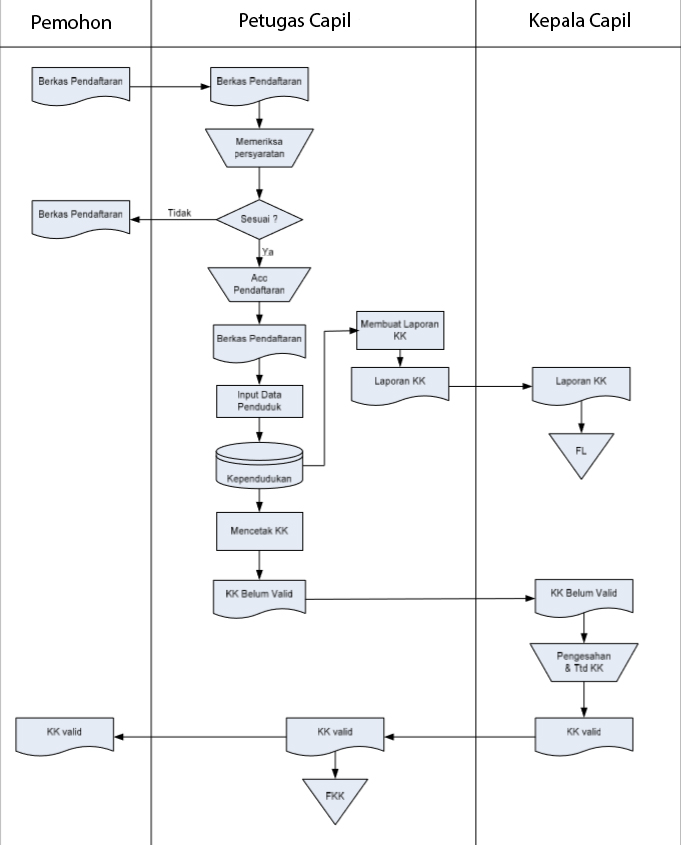
\includegraphics[width=16cm]{figures/flowmap.jpg}
		\caption{Flowmap Prosedur Pembuatan KK.}	
	\end{figure}
\end{enumerate}
\subsection{Syarat-Syarat melakukan Poligami}
\begin{enumerate}
\item Surat permohonan Izin Poligami;
-	Dibuat sebanyak 8 (Delapan).
-	Siapkan Softfile (Flasdisk/CD).
\item Foto Copy KTP Suami dan Istri + Kartu Keluarga;.
\item Foto Copy Buku/ Akta Nikah Pemohon.
\item Surat Pernyataan / Surat Keterangan Penghasilan;.
\item Daftar Harta Kekayaan;.
\item Surat Pernyataan Berlaku Adil.
\item Surat Pernyataan Bersedia Dimadu;.
\section{Pengumpulan Data Fisik}
Data fisik sangat dibutuhkan untuk membuat KK(
Kartu keluarga) untuk Ber-Poligami, adapun Bukti fisiknya sebagai berikut :  
\end{enumerate}
\begin{enumerate}

	\item Kartu Keluarga Keluarga Pertama
	\begin{figure}[H]
		\centering
		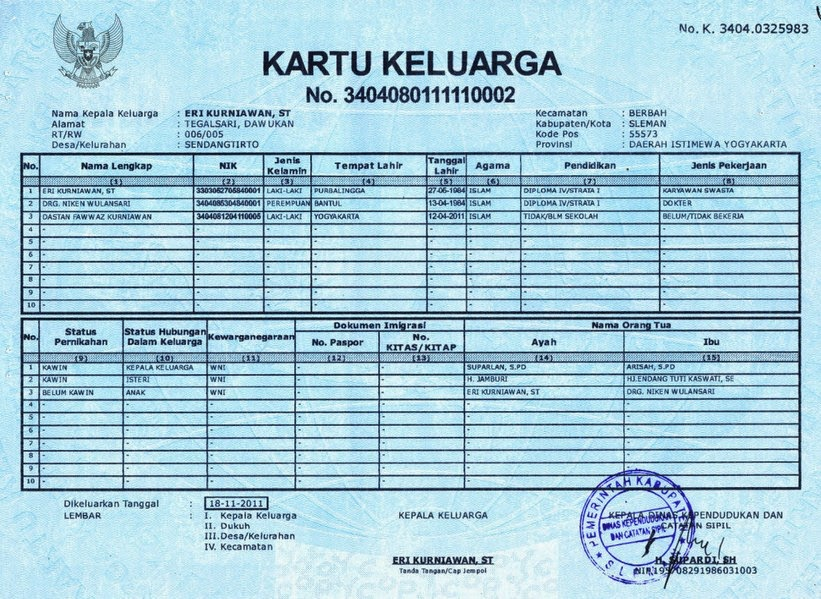
\includegraphics[width=12cm]{figures/kk.jpg}
		\caption{Kartu Keluarga.}	
	\end{figure}

	\item Akta Kelahiran
	\begin{figure}[H]
		\centering
		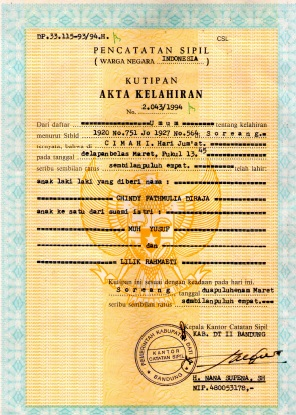
\includegraphics[width=12cm]{figures/akte.jpg}
		\caption{Akta Kelahiran.}	
	\end{figure}

	\item Formulir F-1.21
	\begin{figure}[H]
		\centering
		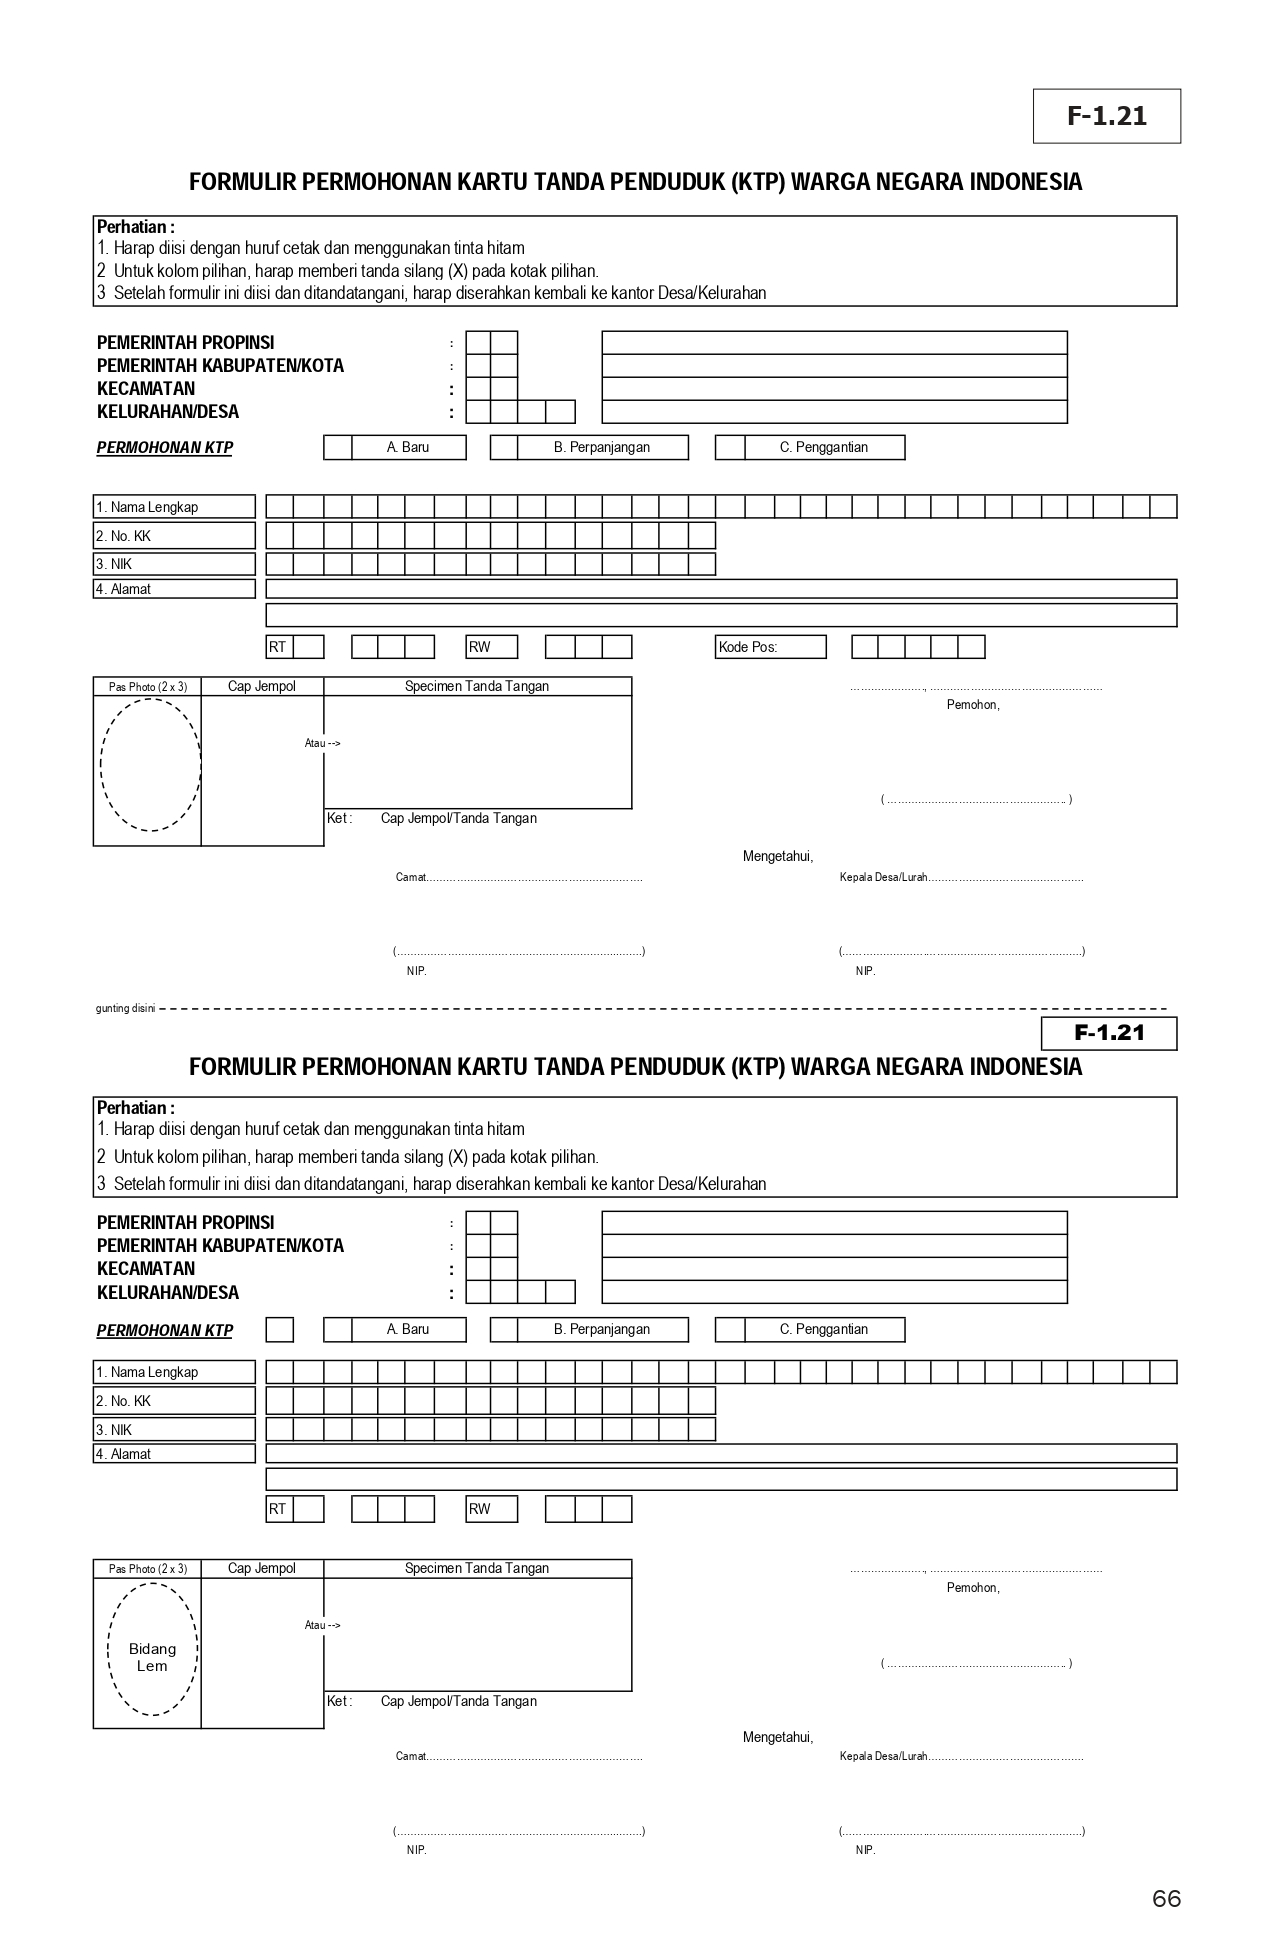
\includegraphics[width=12cm]{figures/formulir.jpg}
		\caption{Formulir F-1.21.}	
	\end{figure}

	\item Surat Pengantar RT dan RW
	\begin{figure}[H]
		\centering
		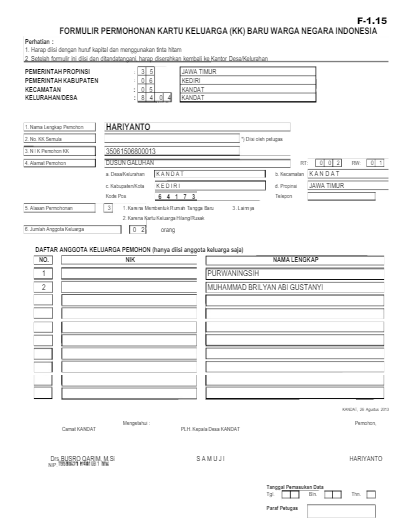
\includegraphics[width=12cm]{figures/surat.png}
		\caption{Surat Pengantar RT dan RW.}	
	\end{figure}

	\item e-KTP
	\begin{figure}[H]
		\centering
		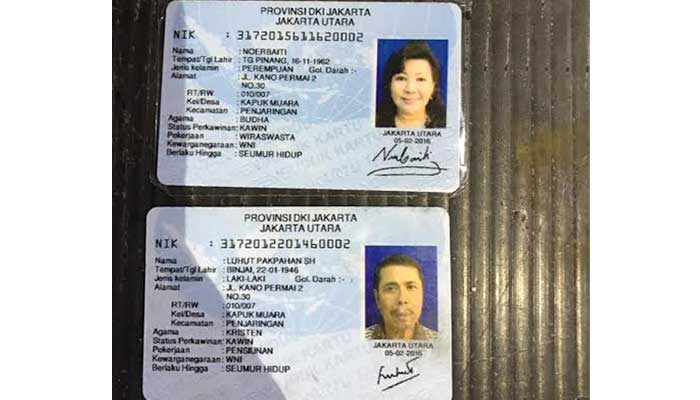
\includegraphics[width=12cm]{figures/ktp.jpg}
		\caption{e-KTP.}	
	\end{figure}

	\item Buku Nikah
	\begin{figure}[H]
		\centering
		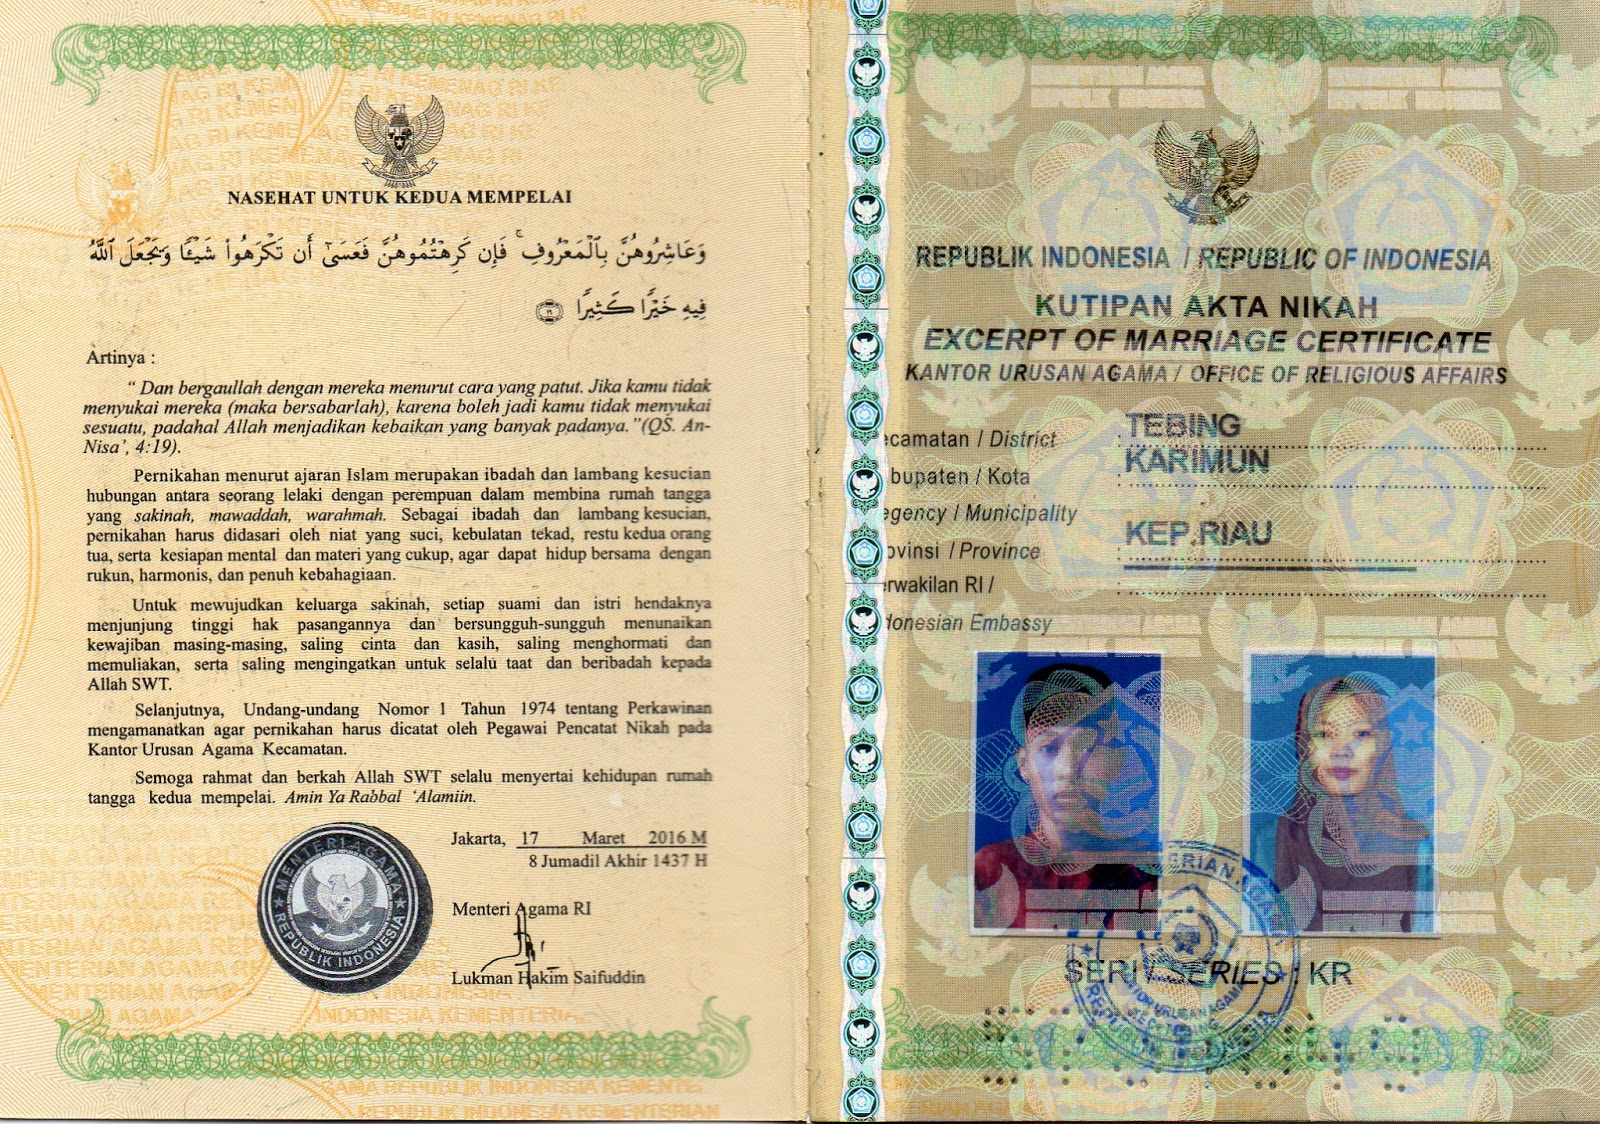
\includegraphics[width=12cm]{figures/bukunikah.jpg}
		\caption{Buku Nikah.}	
	\end{figure}
	
		\item Surat Bersedia Dimadu
	\begin{figure}[H]
		\centering
		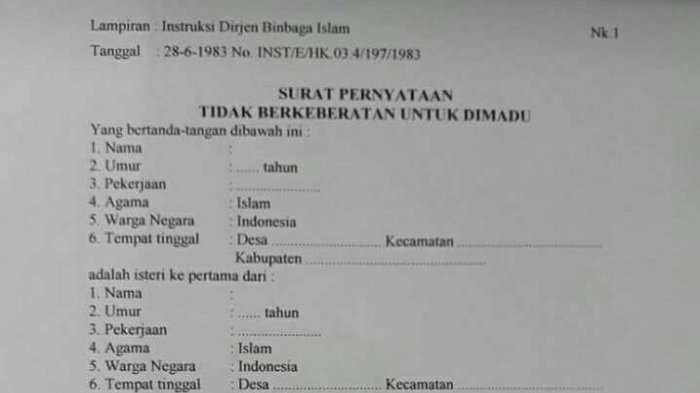
\includegraphics[width=12cm]{figures/surat3.jpg}
		\caption{Surat Bersedia Dimadu.}	
	\end{figure}
	
		\item Surat Bersedia Menjadi Istri Ke-Dua
	\begin{figure}[H]
		\centering
		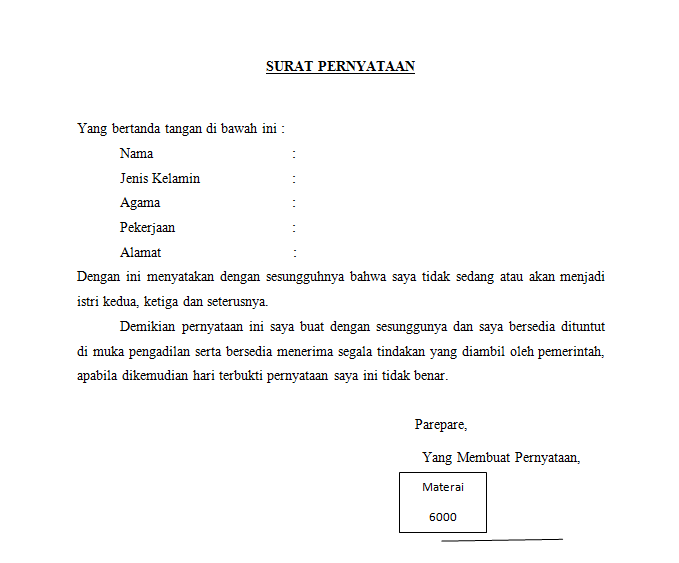
\includegraphics[width=12cm]{figures/surat4.png}
		\caption{Surat Bersedia Menjadi Istri Ke-Dua.}	
	\end{figure}
\end{enumerate}